\documentclass[a4paper]{article}
\usepackage[utf8]{inputenc}
\usepackage{textcomp}
\usepackage{geometry}
\geometry{ left=2cm, right=2cm, top=2cm, bottom=4cm, bindingoffset=5mm}
\usepackage{graphicx}
\usepackage{xcolor}
\usepackage{hyperref}
\date{}
\author{}
\usepackage{fancyhdr}
\pagestyle{fancy}
\fancyhf{}
\fancyhead[R]{3141241 - Jamie Ullerich \\ 2892258 - Gerhard Breul \\ 2973140 - Felix Bühler}
\fancyhead[L]{Information Visualisation and Visual Analytics \\ WS 2019/20 }
\renewcommand{\headrulewidth}{0.5pt}
\usepackage{tikz}
\usetikzlibrary{calc}
\usepackage{amsmath}
\usepackage{cleveref}
\usepackage{subcaption}


\title{\textbf{Assignment 6}}

\begin{document}
\maketitle 
\thispagestyle{fancy}

\section*{Task 1 - Multivariate Data}

\begin{enumerate}
	\item[(a)]
	Yes, there is a correlation between x and y, since the correlation coefficient is very high, there is a positive linear correlation. 
	Surprisingly, the mean, variance and persons correlation coefficient are the same for all four groups. 
	
	
	\begin{tabular}{| c |c c | c c | c c | c c|} \hline
		&\multicolumn{2}{|c|}{I} & \multicolumn{2}{|c|}{II} &
		\multicolumn{2}{c|}{III} & \multicolumn{2}{|c|}{IV} \\ \hline
		&x & y & x & y & x & y & x & y\\ \hline 
		mean & 9 & 7.50 &9 &7.50&9&7.5&9&7.50\\ \hline 
		variance & 11.0 & 4.127 & 11.0 & 4.127  & 11.0 & 4.127 & 11.0 & 4.127 \\ \hline
		pearson & \multicolumn{2}{|c|}{0.8164}  &   \multicolumn{2}{|c|}{0.8164} &  
		 \multicolumn{2}{|c|}{0.8164}  &   \multicolumn{2}{|c|}{0.8164} \\ \hline  
		
	\end{tabular}

	
	\item[(b)] The plots are shown in \Cref{scatterplots} \\
	\begin{figure}[!ht]
		\centering
		\begin{subfigure}{.35\textwidth}
			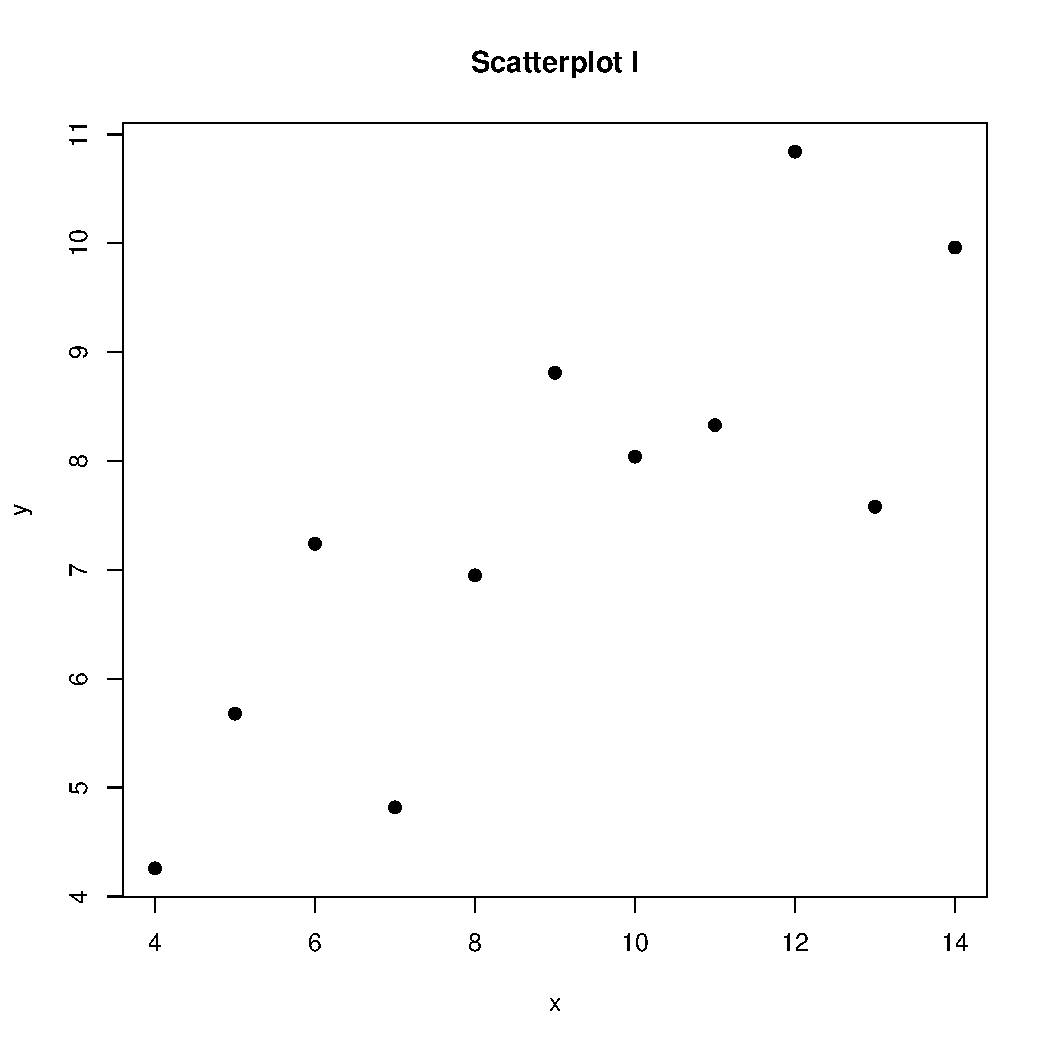
\includegraphics[width=\linewidth]{ScatterplotI.pdf}
		\end{subfigure}		
		\begin{subfigure}{.35\textwidth}
			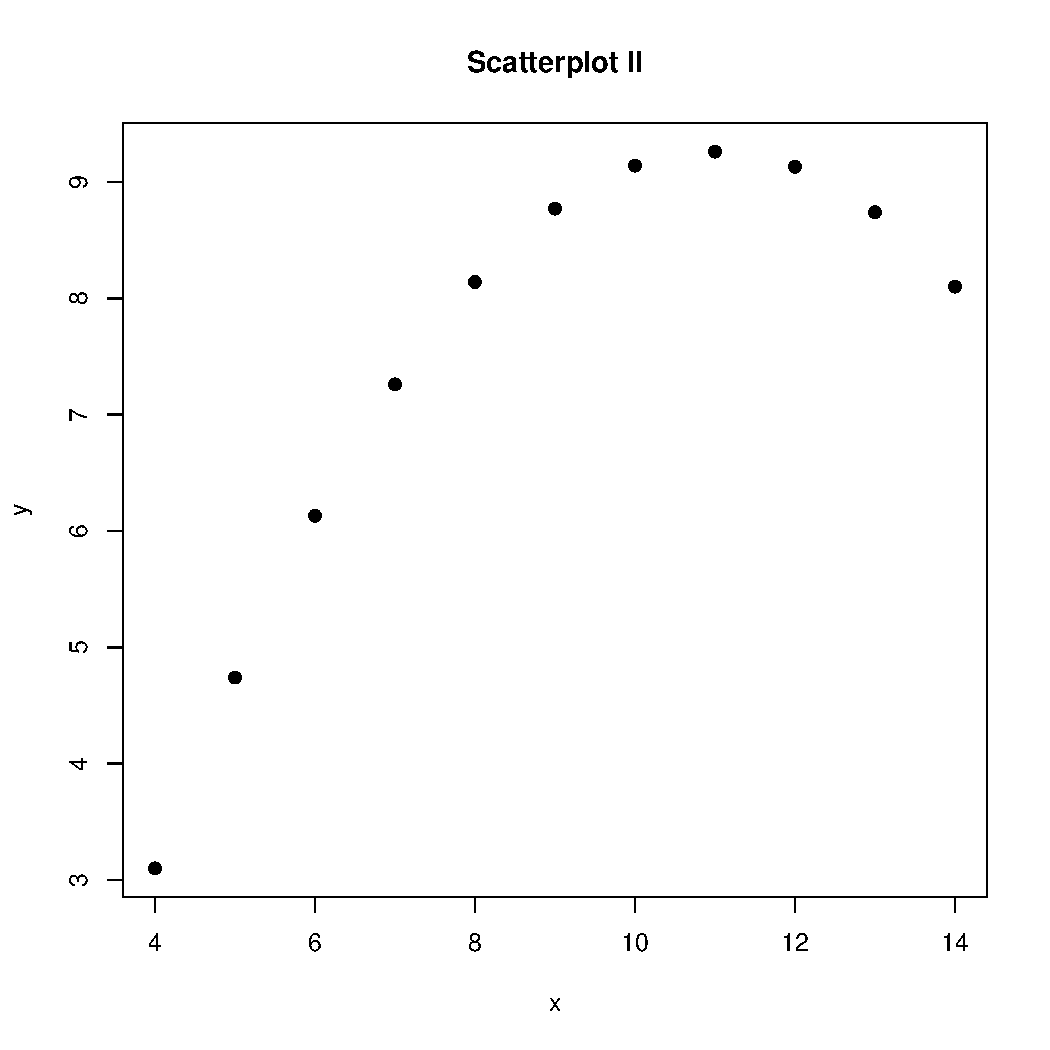
\includegraphics[width=\linewidth]{ScatterplotII.pdf}
		\end{subfigure}
		\begin{subfigure}{.35\textwidth}
			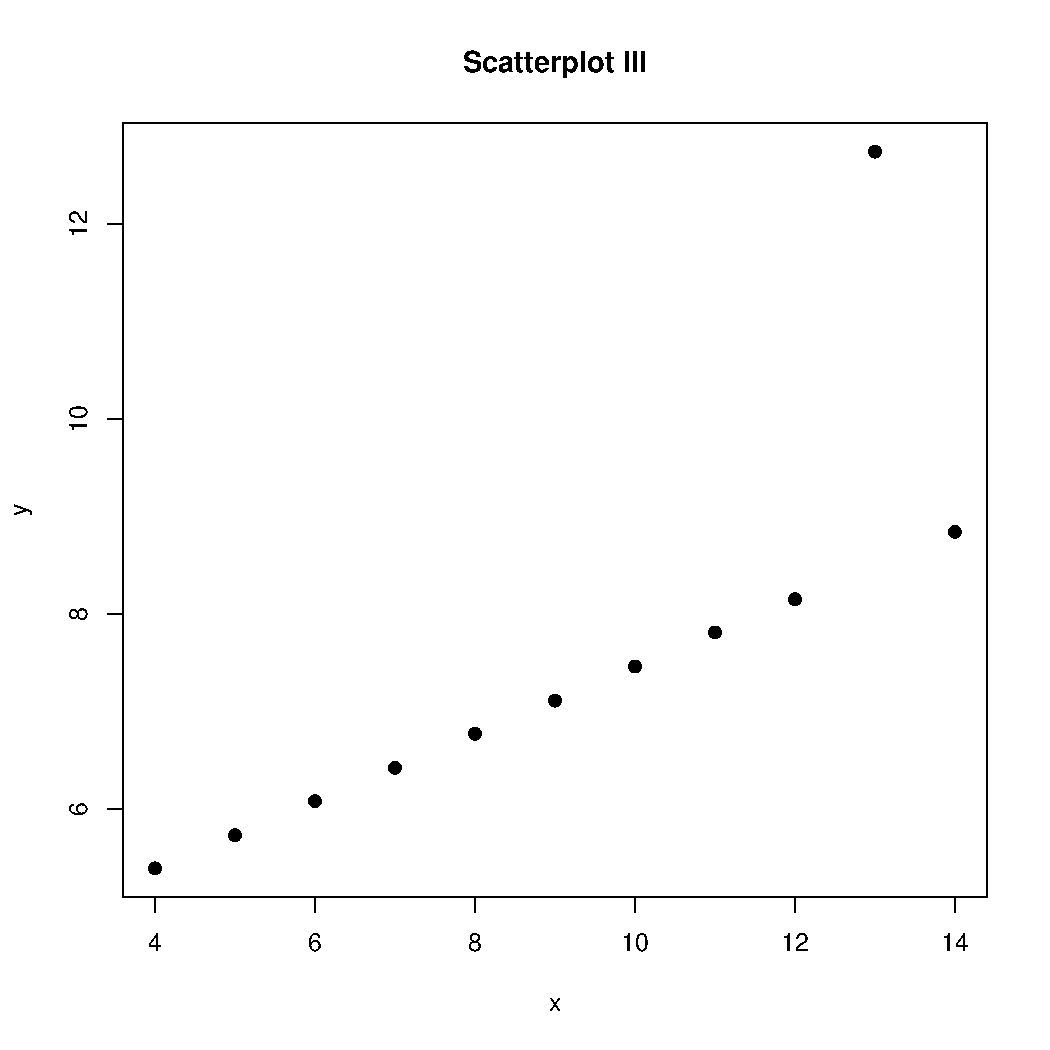
\includegraphics[width=\linewidth]{ScatterplotIII.pdf}
		\end{subfigure}
		\begin{subfigure}{.35\textwidth}
			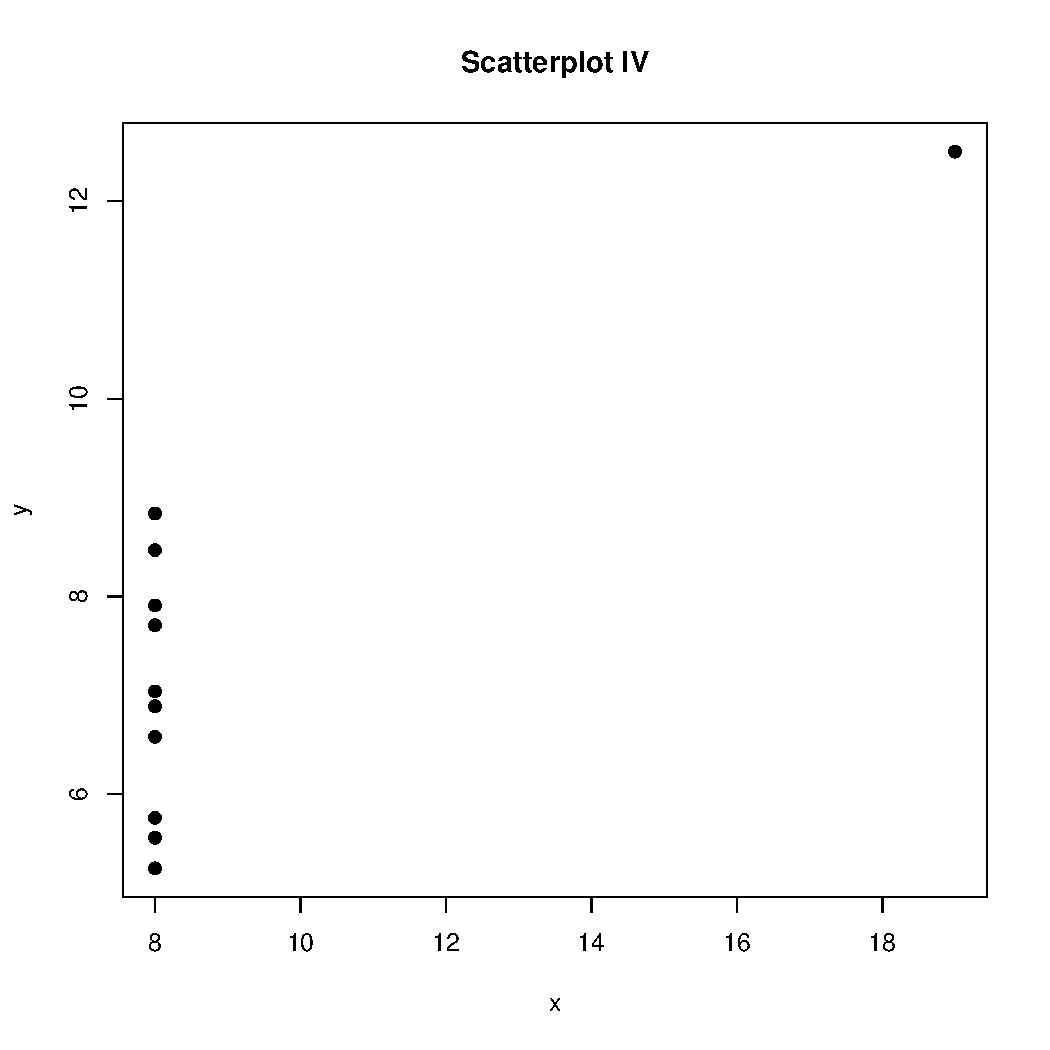
\includegraphics[width=\linewidth]{ScatterplotIV.pdf}
		\end{subfigure}		
		
		
		
		\caption{Task 1 (b) - Scatter plots}
		\label{scatterplots}
	\end{figure}
	
	It is not visible in the plots, that each of these has the same correlation and variance, as well as mean values for x and y. 
	
	\item[(c)] Scatterplot Matrices can be used to visualised this data. 
	This way, the patterns between all variables are still visible and zooming into the plot can be used to see more details. 
	The plot is shown in \Cref{scatterplots_d}.
	\begin{figure}[!ht]
		\includegraphics[width=\linewidth]{task1_d_scatterplot_matrix.png}
		
		\caption{Task 1 (d) - Scatterplot Matrices }
		\label{scatterplots_d}
	\end{figure}
	
\end{enumerate}

\newpage
\section*{Task 2 - Dimensionality Reduction (DR)}

\begin{enumerate}
	\item[a)]Dimensionality reduction is specially useful for reducing computation time and space (storage and memory). Sometime redundant dimensions are causing an overhead, or dimensions can be combined, without loosing information. Also better for visualization, because the user can understand the data.
	\item[b)] See Figure \Cref{fig:rawdata}.
	\begin{figure}[!ht]
		\centering
		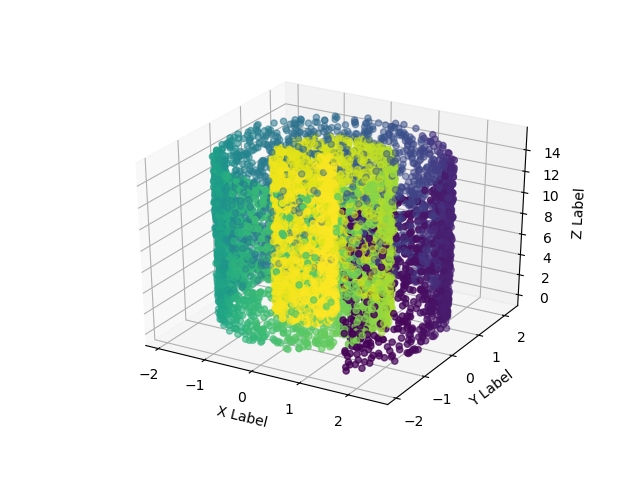
\includegraphics[width=0.7\linewidth]{swiss_roll}
		\caption{raw data}
		\label{fig:rawdata}
	\end{figure}
	\item[c)]
	\begin{itemize}
		\item See \Cref{fig:afterpca}
		
		\begin{figure}[!ht]
			\centering
			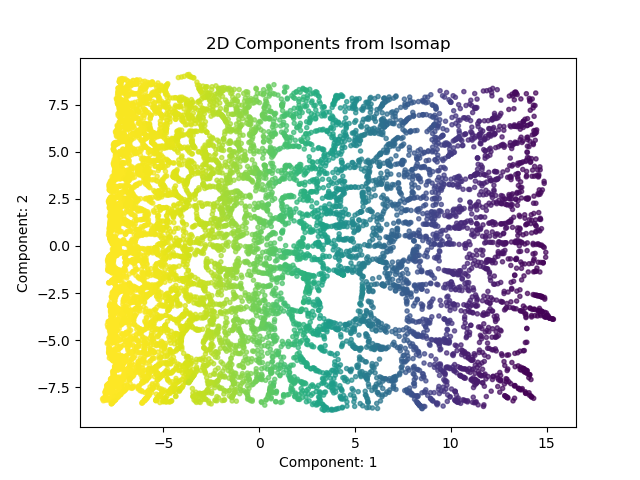
\includegraphics[width=0.7\linewidth]{swiss_roll_result}
			\caption{after pca}
			\label{fig:afterpca}
		\end{figure}
		\item The given spiral is unrolled, so the spiral information is gone missing, but the mat is was made of still preserves the 2d-information.
		%\item TODO
	\end{itemize}
	
\end{enumerate}



-

\end{document}
